\documentclass[11pt]{article}

\usepackage[a4paper,margin=1in]{geometry}
\usepackage{amsmath,amssymb,amsthm}
\usepackage{graphicx}
\usepackage[hidelinks]{hyperref}

\newtheorem{theorem}{Theorem}
\newtheorem{lemma}{Lemma}
\newtheorem{corollary}{Corollary}

\newcommand{\N}{\mathbb{N}}
\newcommand{\eps}{\varepsilon}
\newcommand{\conv}{\operatorname{conv}}
\newcommand{\diam}{\operatorname{diam}}
\newcommand{\norm}[1]{\left\lVert #1 \right\rVert}
\newcommand{\abs}[1]{\left\lvert #1 \right\rvert}

\title{The Fixed-Epsilon Renorming From arXiv:2301.07943 Is Not LASQ}
\author{Automatic math-discovery smoke test}
\date{June 15, 2026}

\begin{document}
\maketitle

\section*{Source Problem}

The source paper is Jose Rodriguez and Abraham Rueda Zoca,
\emph{On weakly almost square Banach spaces}, arXiv:2301.07943
\cite{RodriguezRuedaZoca2023}.  On page 3 of the arXiv PDF, after recalling
that slice-D2P and D2P are distinct, the authors ask whether there exists a
locally almost square (LASQ) Banach space which fails D2P.

\begin{center}
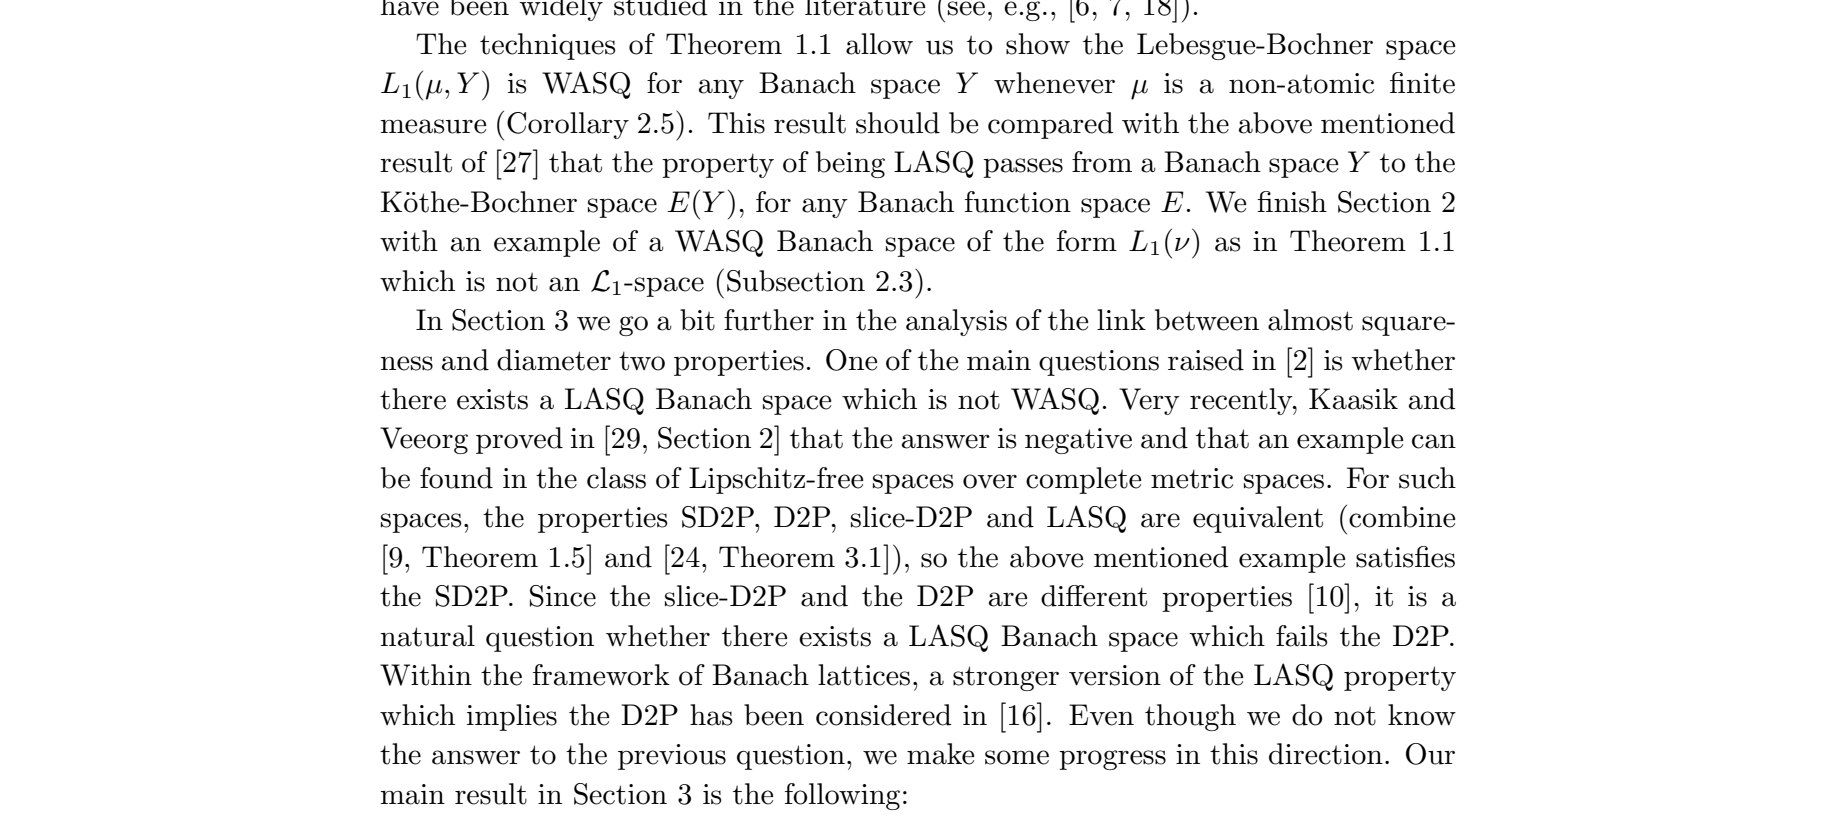
\includegraphics[width=\linewidth]{figures/open_question_crop_page3.png}
\end{center}

Their Theorem 1.2, shown below from page 4, proves a near-square renorming
result for spaces containing a complemented copy of \(c_0\).

\begin{center}
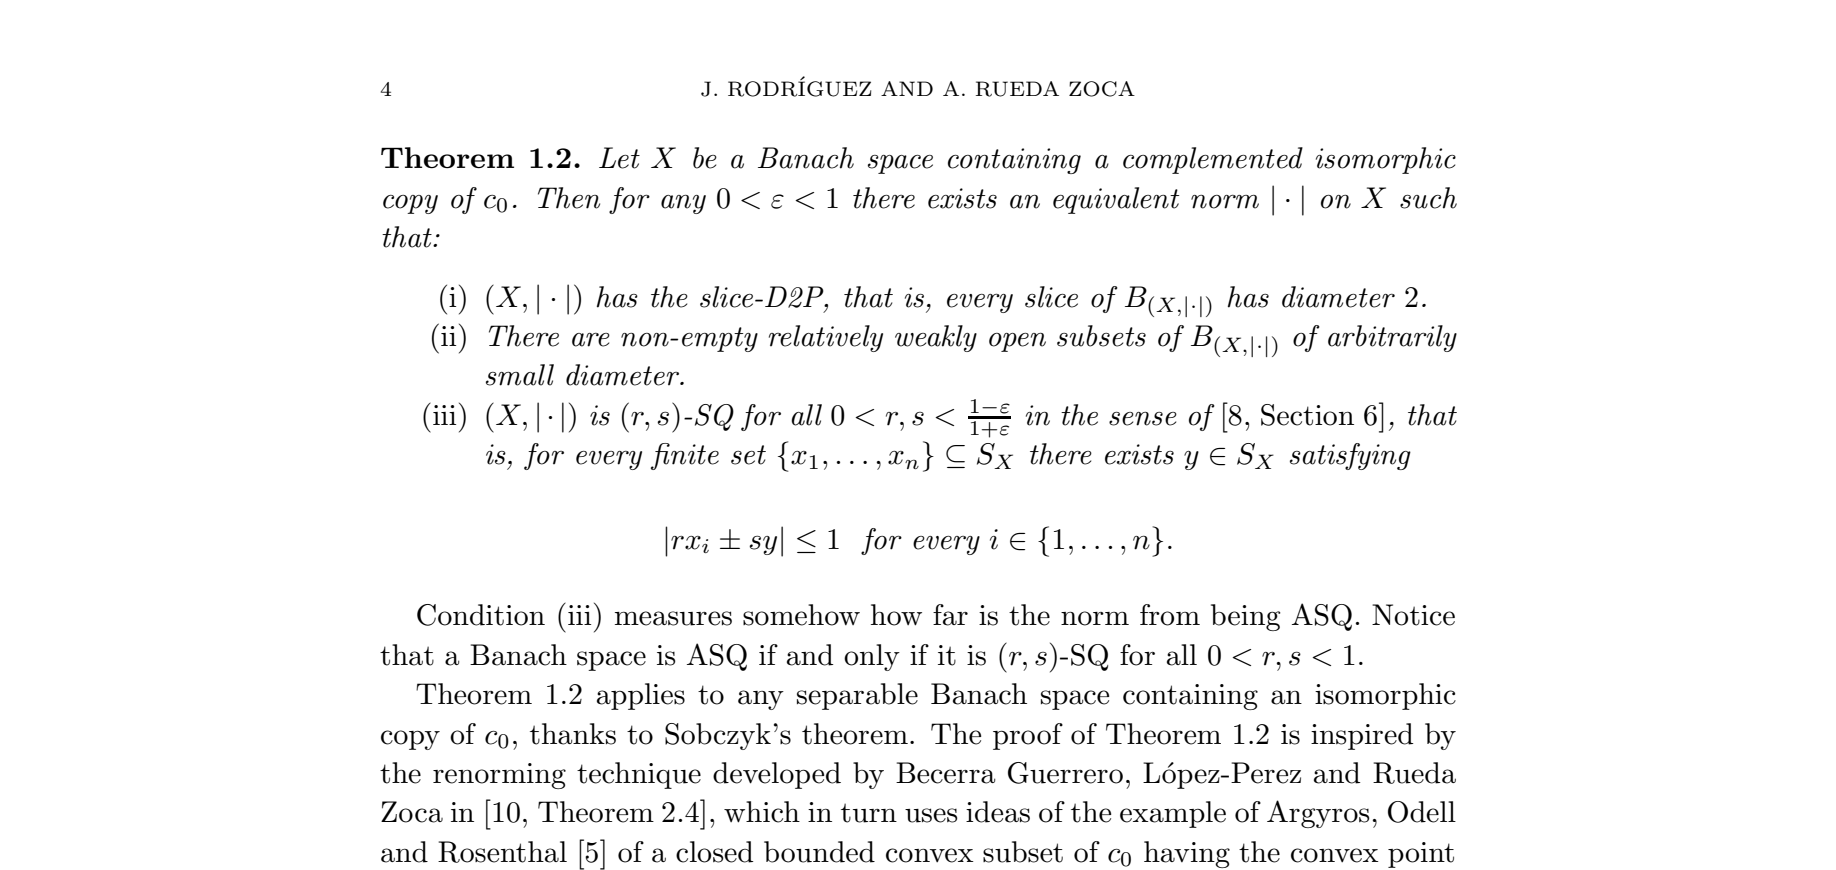
\includegraphics[width=\linewidth]{figures/theorem_1_2_crop_page4.png}
\end{center}

\section*{Result Type}

This packet gives a \textbf{partial obstruction}.  It proves that the concrete
fixed-\(\eps\) renorming used in the source proof of Theorem 1.2 is not LASQ.
Thus the paper's construction cannot itself be the desired LASQ space failing
D2P.  The full LASQ-versus-D2P question remains open.

\section*{Proof Intuition}

The source unit ball is built from three kinds of generators.  The first two,
\(A\times\{0\}\) and \(-A\times\{0\}\), have no second \(c_0\)-coordinate.  The
third kind can carry second-coordinate mass, but only after paying a fixed
positive \(\eps\) in the functional \(L=(\lim,0)\): those points have
\(L\geq -(1-\eps)\), whereas the tree points \(x_\alpha\in A\) have
\(L=-1\).  Consequently, any point of the unit ball with \(L\) very close to
\(-1\) has very small second coordinate.  At the particular point
\((x_\emptyset,0)\), the first coordinate is already coordinatewise on the
boundary of the ambient sup-norm ball.  If both \((x_\emptyset,0)\pm y\) stay
almost in the unit ball, then both the first and second coordinates of \(y\)
must be small.  This makes \((x_\emptyset,0)\) strongly extreme, which is
incompatible with LASQ.

\section*{Definitions And Source Construction}

We use the notation of Section 3 of the source paper.  Let
\[
Z=c(\N^{<\omega})\oplus_\infty c_0
\]
with its usual norm \(\norm{\cdot}_Z\).  For each
\(\alpha\in\N^{<\omega}\), define \(x_\alpha\in c(\N^{<\omega})\) by
\[
x_\alpha(\beta)=
\begin{cases}
1, & \beta\preceq \alpha,\\
-1, & \text{otherwise}.
\end{cases}
\]
Put \(A=\{x_\alpha:\alpha\in\N^{<\omega}\}\).  The source fixed-\(\eps\)
unit ball is
\[
B=\overline{\conv}\Big( (A\times\{0\})\cup (-A\times\{0\})\cup
\big((1-\eps)B_Z+\eps B_{c_0(\N^{<\omega})}\times\{0\}\big)\Big),
\]
where \(0<\eps<1\).  Let \(\abs{\cdot}\) be the Minkowski functional of \(B\).
The source proof notes that
\[
(1-\eps)B_Z\subseteq B\subseteq B_Z,
\quad\text{hence}\quad
\norm{z}_Z\leq \abs{z}\leq \frac{1}{1-\eps}\norm{z}_Z.
\]
Let \(P_2:Z\to c_0\) be the second-coordinate projection and let
\[
L(x,y)=\lim x.
\]

A point \(p\in S_{(Z,\abs{\cdot})}\) is strongly extreme if
\(\abs{p\pm y_n}\to 1\) implies \(\abs{y_n}\to 0\).

\section*{Main Result}

\begin{lemma}\label{lem:second-coordinate-bound}
For every \(w\in B\),
\[
\norm{P_2 w}_\infty
\leq
\frac{1-\eps}{\eps}\bigl(1+L(w)\bigr).
\]
\end{lemma}

\begin{proof}
Consider first the three generating pieces of \(B\).
If \(w\in A\times\{0\}\) or \(w\in -A\times\{0\}\), then
\(P_2w=0\), so the inequality is immediate.  If
\[
w=(1-\eps)u+\eps(v,0)
\]
with \(u\in B_Z\) and \(v\in B_{c_0(\N^{<\omega})}\), then
\[
\norm{P_2w}_\infty\leq 1-\eps
\]
and
\[
L(w)=(1-\eps)L(u)\geq -(1-\eps).
\]
Therefore \(1+L(w)\geq \eps\), and the desired inequality again holds.

The set of \(w\in Z\) satisfying the displayed inequality is convex: the left
side is convex and the right side is affine.  It is also norm closed.  Since it
contains all generators, it contains their closed convex hull \(B\).
\end{proof}

\begin{theorem}\label{thm:not-lasq}
For every \(0<\eps<1\), the fixed-\(\eps\) renormed space
\((Z,\abs{\cdot})\) constructed in the source proof is not LASQ.  In fact,
\(p=(x_\emptyset,0)\) is a strongly extreme point of \(B\).
\end{theorem}

\begin{proof}
First note that \(p\in S_{(Z,\abs{\cdot})}\): \(p\in A\times\{0\}\subseteq B\),
while \(B\subseteq B_Z\) and \(\norm{p}_Z=1\).

Let \(y=(u,v)\in Z\), and suppose that
\[
\abs{p+y}\leq 1+\delta,
\qquad
\abs{p-y}\leq 1+\delta
\]
for some \(\delta\geq 0\).  Since \(B\subseteq B_Z\), we have
\[
\norm{x_\emptyset\pm u}_\infty\leq 1+\delta.
\]
Every coordinate of \(x_\emptyset\) has absolute value \(1\).  Hence
\(\abs{u(\beta)}\leq \delta\) for every \(\beta\in\N^{<\omega}\), so
\[
\norm{u}_\infty\leq \delta
\quad\text{and}\quad
\abs{\lim u}\leq \delta.
\]

Set \(q_+=(p+y)/(1+\delta)\in B\).  Lemma
\ref{lem:second-coordinate-bound} gives
\[
\frac{\norm{v}_\infty}{1+\delta}
=\norm{P_2q_+}_\infty
\leq
\frac{1-\eps}{\eps}
\left(1+\frac{-1+\lim u}{1+\delta}\right)
=
\frac{1-\eps}{\eps}\,
\frac{\delta+\lim u}{1+\delta}
\leq
\frac{1-\eps}{\eps}\,
\frac{2\delta}{1+\delta}.
\]
Thus
\[
\norm{v}_\infty\leq \frac{2(1-\eps)}{\eps}\delta.
\]
Combining the two coordinate estimates,
\[
\norm{y}_Z
\leq
\max\left\{\delta,\frac{2(1-\eps)}{\eps}\delta\right\}.
\]
Using the source norm comparison,
\[
\abs{y}
\leq
\frac{1}{1-\eps}\norm{y}_Z
\leq
\max\left\{\frac{1}{1-\eps},\frac{2}{\eps}\right\}\delta.
\]

Now let \(y_n\in Z\) be any sequence such that
\(\abs{p+y_n}\to 1\) and \(\abs{p-y_n}\to 1\).  Applying the estimate with
\[
\delta_n=\max\{\abs{p+y_n},\abs{p-y_n}\}-1
\]
gives \(\abs{y_n}\to 0\).  Therefore \(p\) is strongly extreme.

An LASQ space cannot have this behavior at a sphere point: LASQ would require
a sequence \(y_n\in B\) with \(\abs{p\pm y_n}\to 1\) and
\(\abs{y_n}\to 1\).  Hence \((Z,\abs{\cdot})\) is not LASQ.
\end{proof}

\begin{corollary}
The fixed-\(\eps\) construction in the proof of Theorem 1.2 of
\cite{RodriguezRuedaZoca2023} cannot by itself provide a locally almost square
Banach space failing D2P.
\end{corollary}

\begin{proof}
The theorem shows that the core \(c_0\)-renorming used in the construction is
not LASQ for any fixed \(0<\eps<1\).
\end{proof}

\section*{Verification Notes}

No numerical computation is used.  The only estimate requiring review is
Lemma \ref{lem:second-coordinate-bound}.  It is a generator-by-generator
convexity estimate: second-coordinate mass can occur only in the third
generating piece, and that piece raises the \(L=(\lim,0)\) value by at least
\(\eps\) from the tree value \(-1\).

\section*{Limitations And Novelty Check}

This packet does not solve the full question whether there exists a LASQ
Banach space failing D2P.  It rules out only the most direct attempt to upgrade
the source fixed-\(\eps\) renorming to LASQ.  It also does not rule out
renormings with a variable parameter, different tree balls, or non-\(c_0\)
constructions.

Before packaging, the run's lightweight indexes were searched for
arXiv:2301.07943, the paper title, weakly almost square, locally almost square,
LASQ, WASQ, D2P, and diameter two phrases.  No duplicate packet for this
paper or this obstruction was found.  A bounded web search on June 15, 2026
for exact phrases including \(\text{``locally almost square''}\)
\(\text{``diameter two property''}\), \(\text{``LASQ''}\)
\(\text{``D2P''}\), and close variants found the source paper and nearby
LASQ lattice/transfinite-ASQ papers, but no later explicit answer to the full
LASQ-fails-D2P question.

\section*{Human Review Recommendation}

The proof is short and appears likely valid.  Reviewers should verify that the
closed convex hull argument in Lemma \ref{lem:second-coordinate-bound} is
legitimate and that the coordinatewise boundary argument for
\(x_\emptyset\) indeed forces \(\norm{u}_\infty\leq\delta\) whenever
\(p\pm(u,v)\in (1+\delta)B\).

\begin{thebibliography}{9}

\bibitem{RodriguezRuedaZoca2023}
J.~Rodriguez and A.~Rueda Zoca,
\emph{On weakly almost square Banach spaces},
arXiv:2301.07943, 2023.

\bibitem{AbrahamsenLangemetsLima2015}
T.~A. Abrahamsen, J.~Langemets, and V.~Lima,
\emph{Almost square Banach spaces},
Journal of Mathematical Analysis and Applications 434 (2016), 1549--1565.

\end{thebibliography}

\end{document}
